% $> xelatex spsi.tor.presentacion.tex
% o bien
% $> lualatex spsi.tor.presentacion.tex
\documentclass[spanish]{beamer}

\usepackage{babel}

\usepackage{graphics,tikz}
\usetikzlibrary{automata, positioning, arrows}

\usepackage{pgfplotstable}
\pgfplotsset{compat=1.16}

\usepackage{adjustbox}

\usepackage{enumitem}

%%% FUENTES

\usepackage[no-math]{fontspec}
\setsansfont{Fira Sans}
\setromanfont{Libertinus Serif}
\setmonofont[Scale=.9]{Fira Mono}

\usepackage[math-style=TeX]{unicode-math}
\setmathfont{Fira Math}

\usepackage{pifont}
\newcommand{\cmark}{\ding{51}}%
\newcommand{\xmark}{\ding{55}}%

%%% COLORES

\definecolor{background}{HTML}{F5F5F4}
\definecolor{foreground}{HTML}{3F3F3F}
\definecolor{strings}{HTML}{ED982C}
\definecolor{operators}{HTML}{CF4818}
\definecolor{identifiers}{HTML}{9A71BA}
\definecolor{keywords}{HTML}{5486C8}
\definecolor{numbers}{HTML}{80951D}
\definecolor{comments}{HTML}{AFAFAF}

%%% LISTINGS

\usepackage{listings}

\lstset{
  numbers=left,
  belowcaptionskip=1\baselineskip,
  basicstyle=\scriptsize\ttfamily\color{foreground},
  keywordstyle=\color{keywords},
  commentstyle=\color{comments},
  stringstyle=\color{strings},
  identifierstyle=\color{identifiers},
  numberstyle=\color{foreground},
  xleftmargin=2em,
  framexleftmargin=1.5em,
  breaklines=true,
  showstringspaces=false,
  tabsize=2
}

%%% AJUSTES DE BEAMER

%\usefonttheme{professionalfonts}

\setbeamertemplate{navigation symbols}{}

\setbeamerfont{title}{series=\bfseries}

%\setbeamertemplate{frametitle}{\color{foreground}\vspace*{1cm}\bfseries\insertframetitle\par\vskip-6pt}
\setbeamerfont{frametitle}{series=\bfseries}
\setbeamercolor{frametitle}{fg=foreground}
\setbeamerfont{framesubtitle}{size=\normalfont\small}
\setbeamercolor{framesubtitle}{fg=foreground}

\setbeamercolor{background canvas}{bg=background}

\setbeamercolor{normal text}{fg=foreground}
\setbeamercolor{alerted text}{fg=foreground}
\setbeamercolor{block title}{fg=foreground}
\setbeamercolor{alerted text}{fg=foreground}

\setbeamercolor{itemize item}{fg=foreground}
\setbeamercolor{enumerate item}{fg=foreground}

\setbeamertemplate{itemize items}[circle]
\setitemize{
  label=\usebeamerfont*{itemize item}
  \usebeamercolor[fg]{itemize item}
  \usebeamertemplate{itemize item}
}

\setbeamercolor*{title}{fg=foreground}
\setbeamercolor{qed symbol}{fg=foreground}

\usebeamercolor[fg]{normal text}

%%% INFORMACIÓN DEL DOCUMENTO

\title{La red Tor}
\subtitle{Seguridad y Protección de Sistemas Informáticos}
\author{
  José María Martín Luque \texorpdfstring{\\}{}
  Antonio Martín Ruiz \texorpdfstring{\\}{}
  Daniel Pozo Escalona
}

\begin{document}

\maketitle

\begin{frame}{¿Qué es Tor?}

\end{frame}

\section{Algoritmos de cifrado de Tor}

\begin{frame}{Estructura de la red Tor}

Formada por nodos que se comunican mediante TCP/IP

  \begin{enumerate}

    \item Nodos medios

    \item Nodos salida

    \item Puentes

  \end{enumerate}

\end{frame}

\begin{frame}{Enrutamiento cebolla}

\begin{figure}[h]
  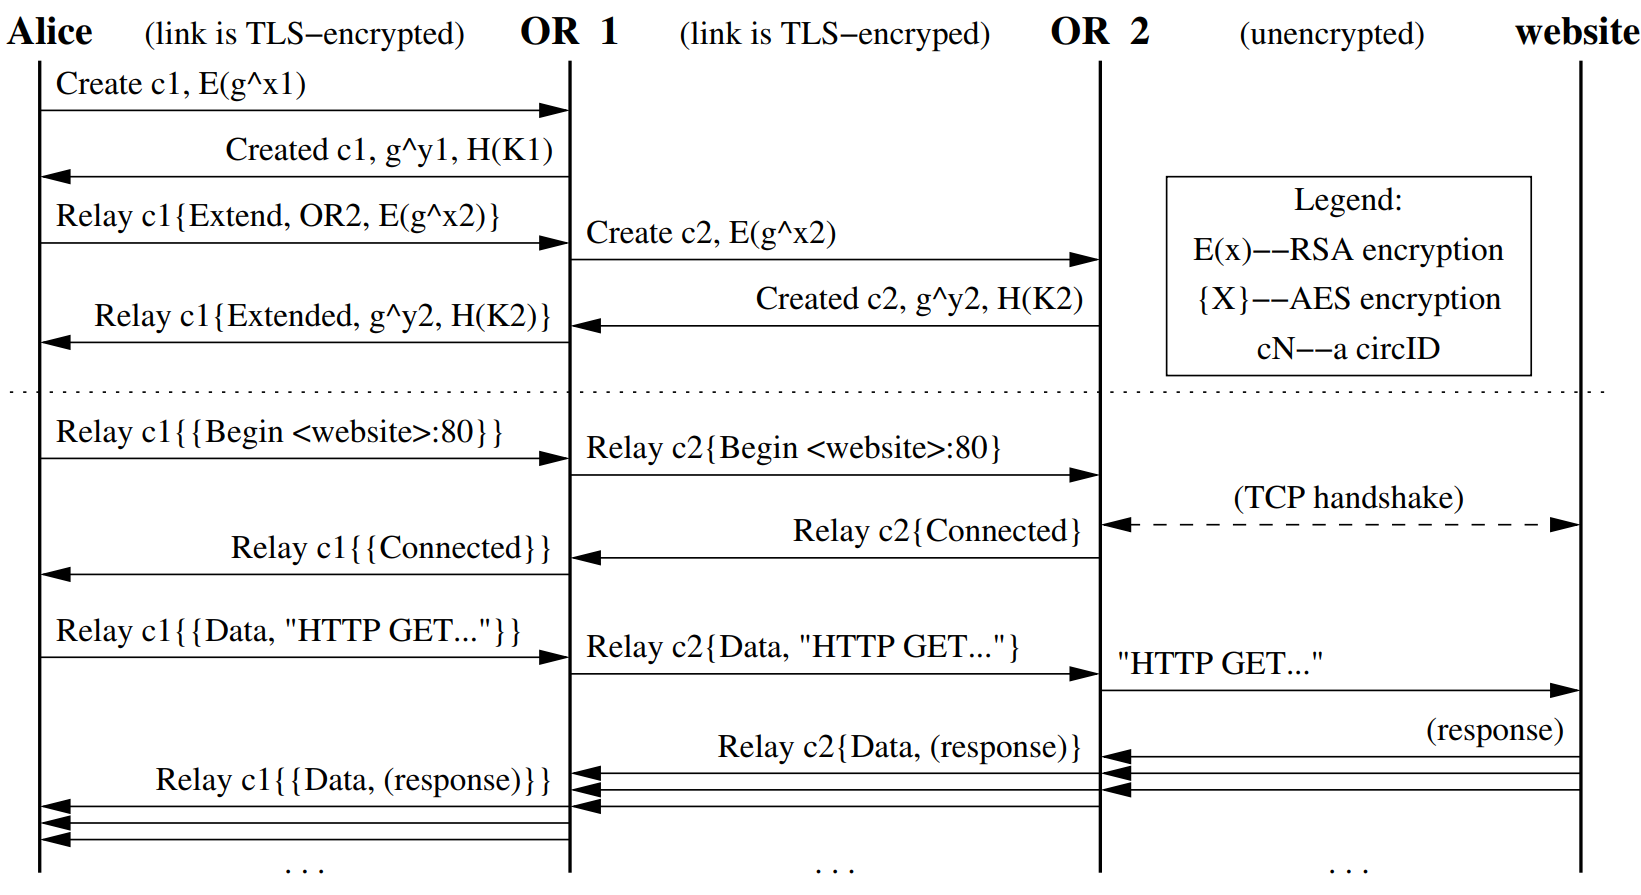
\includegraphics[width=\textwidth]{OR5.png}
  \caption{Diagrama representando un ejemplo de comunicación entre una usuaria (Alice) y una página web, pasando por dos nodos intermedios.}
  \label{fig:or5}
\end{figure}

\end{frame}

\begin{frame}{Enrutamiento cebolla}

\begin{figure}[h]
  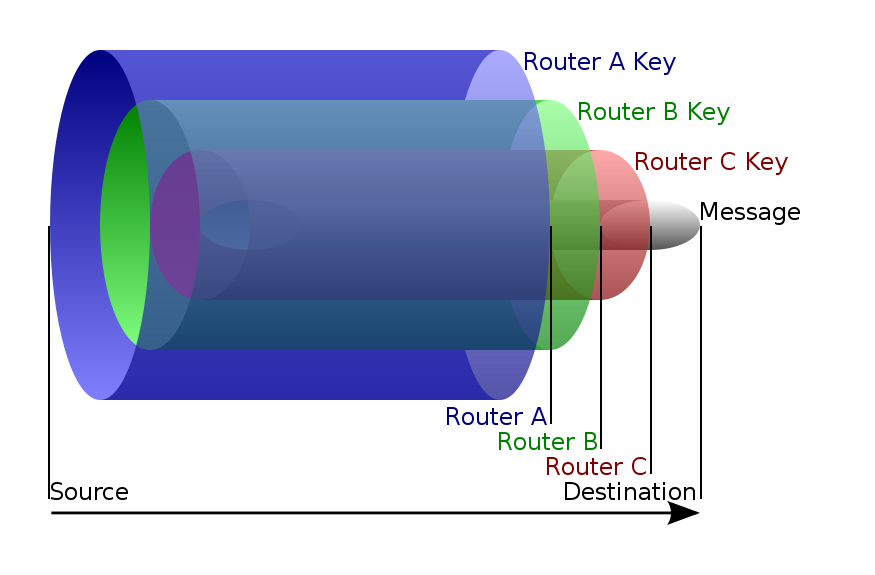
\includegraphics[width=\textwidth]{OR4.png}
  \label{fig:or4}
\end{figure}

\end{frame}

\section{Algoritmos de cifrado de Tor}

\begin{frame}{Algoritmos de cifrado de Tor}{}

  \begin{itemize}
    \item Las conexiones usan TLS/SSLv3

    \item Permite elegir suite de cifrado

    \item TLS tiene dos fases \begin{enumerate}
      \item Establecimiento de la comunicación: determinar una clave compartida
      \item Intercambio de información
    \end{enumerate}
  \end{itemize}

\end{frame}

\begin{frame}{Algoritmos de cifrado de Tor}{Establecimiento de la conexión}

  \begin{itemize}
    \item Inicialmente se usaba un protocolo llamado TAP. \begin{itemize}
      \item Diffie-Hellman clásico sobre un cuerpo finito de orden \[
        p = 2^{1024} - 2^{960} - 1 + 2^{64} \cdot \left\lfloor (2^{894} \pi) + 129093 \right\rfloor.
      \]
      \item Se demostró que tenía deficiencias.
    \end{itemize}
    \item Se creó entonces \textit{ntor}, que usa ECDH. \begin{itemize}
      \item Diffie-Hellman sobre el grupo generado por la curva \textit{Curve25519}, de ecuación \[y^{2}=x^{3}+486662x^{2}+x\] sobre el cuerpo finito de orden el primo \(2^{255}-19\).
    \end{itemize}
  \end{itemize}

\end{frame}

\begin{frame}{Algoritmos de cifrado de Tor}{Intercambio de datos}

  \begin{itemize}
    \item Una vez establecida la conexión y determinada la clave, se usa AES.
  \end{itemize}

\end{frame}

\end{document}
